\chapter{Implementation}

This chapter focus on the implementation details of two add-ons:
\begin{enumerate}
\item a malicious add-on, which can infect the victim`s filesystem.
\item a Transcriptase detection add-on, which can detect the metamorphic malware embedded in the web page.
\end{enumerate}

\section{Malicious add-on}

Generally browsers like Firefox, Chrome, and Opera do not allow access to the client filesystem using JavaScript. Even though creating a file is possible in IE using ActiveX objects, the client must enable ActiveX scripts on their system for the ActiveX object related code to execute properly \cite{bib17}. 

Firefox add-ons are very powerful because of the high-level APIs that the SDK provides. The SDK has a file I/O module which provides access to the client`s filesystem.

A malicious add-on was created to demonstrate the way that a victim`s machine may get infected by a malicious add-on. The basic functionality of this add-on is it provides the statistic value i.e., the total JavaScript bytes in the page loaded by the user, as shown in Figure ~\ref{fig:maliciousaddon}.

\begin{figure}
    \centering    
    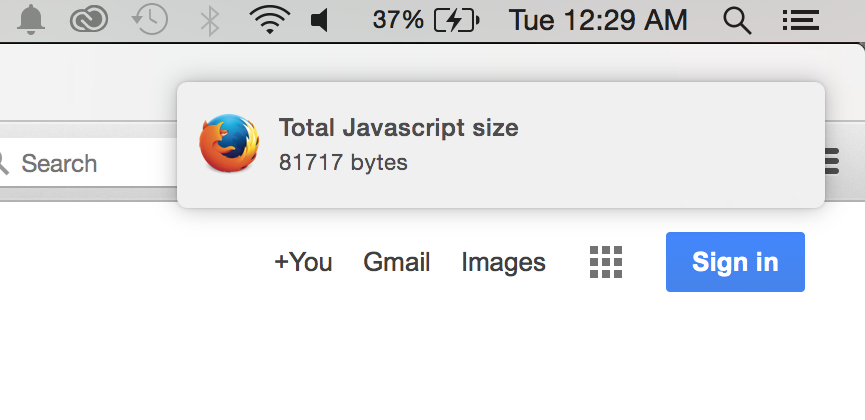
\includegraphics[width=8cm, height=3.9cm]{maliciousaddon.png}
    \caption[Main Functionality of the malicious add-on]{Main Functionality of the malicious add-on}
    \label{fig:maliciousaddon}
\end{figure}

The user expects this functionality and installs the malicious add-on, but this add-on also has hidden functionality. Whenever it finds that web page content has Transcriptase in it, it finds all the JavaScript files present in the filesystem and prepends them with Transcriptase code and thus it infects the victim`s filesystem. 

\begin{figure}
    \centering    
    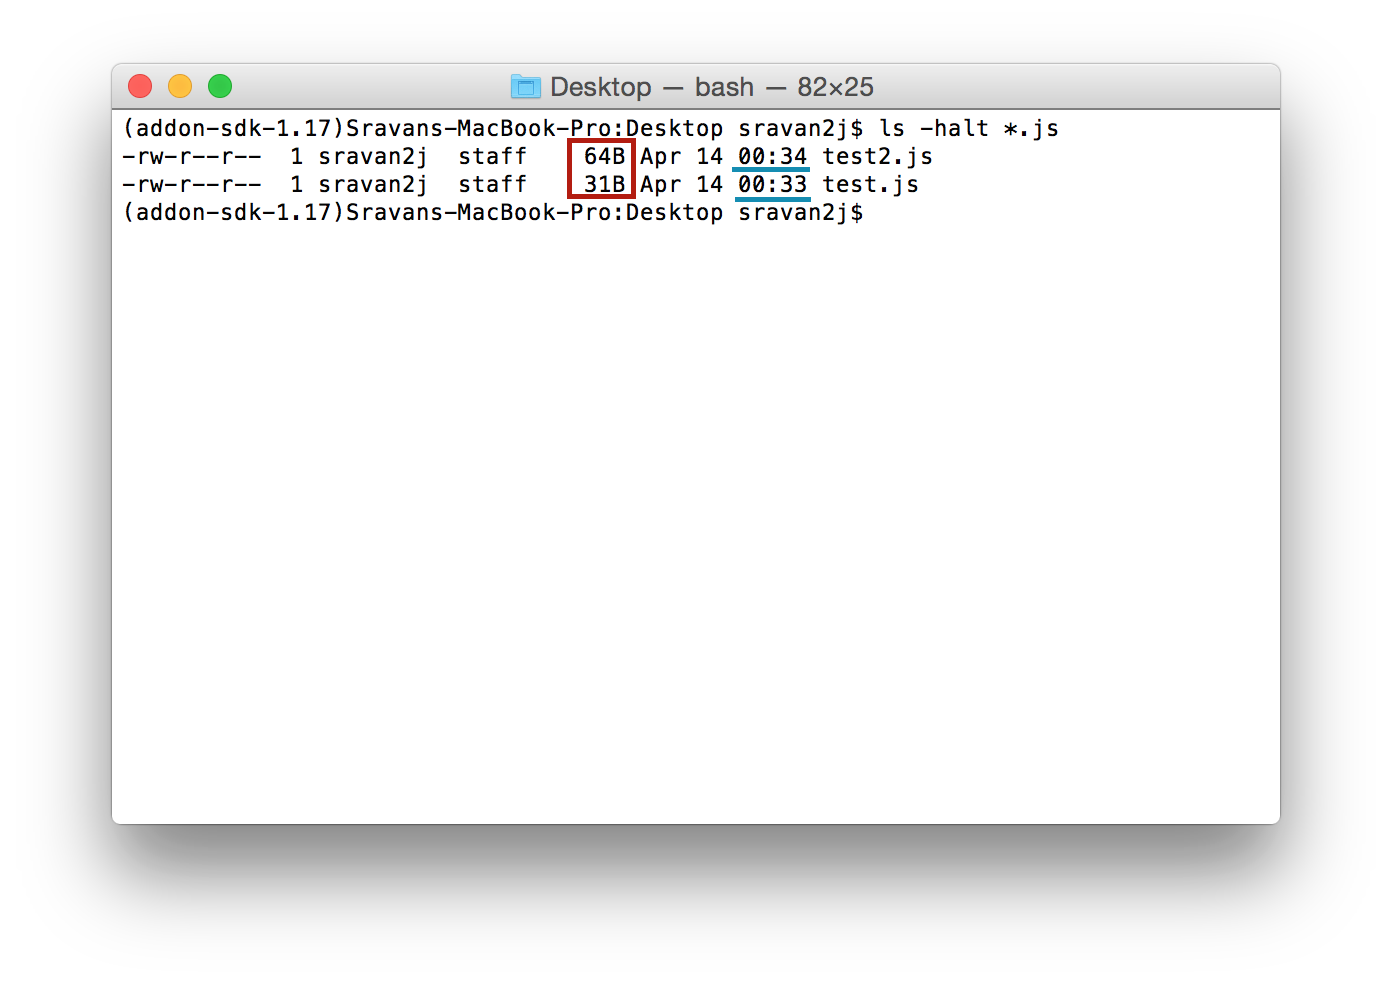
\includegraphics[width=17cm, height=11.95cm]{beforeinf.png}
    \caption[Size of sample JavaScript files before infection, ]{Size of sample JavaScript files before infection}
    \label{fig:beforeinf}
\end{figure}
\begin{figure}
    \centering    
    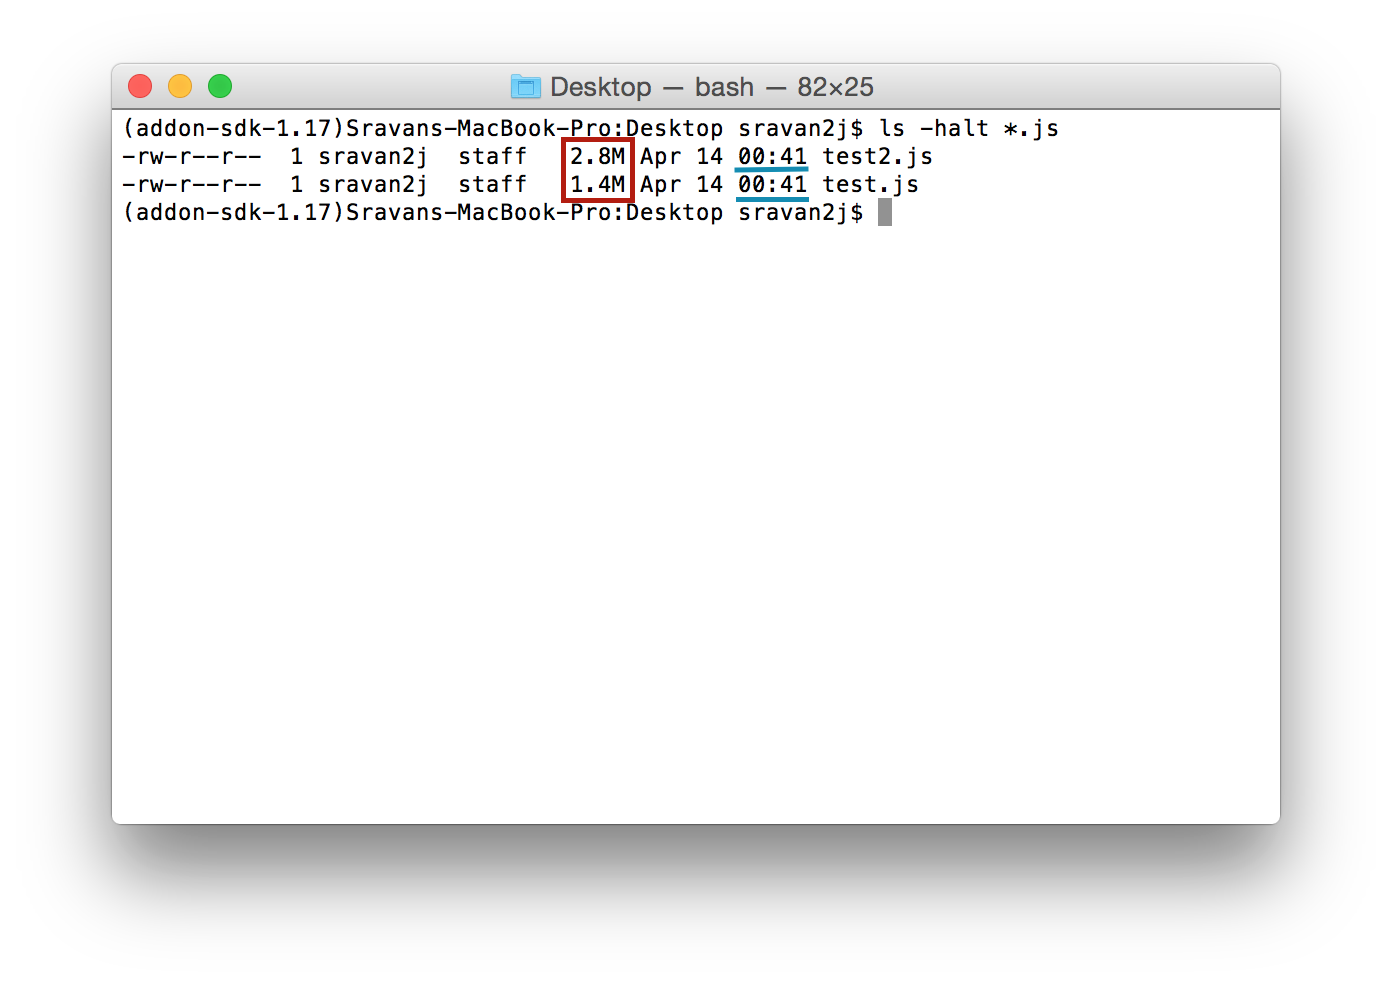
\includegraphics[width=17cm, height=11.95cm]{afterinf.png}
    \caption[JavaScript file sizes after infection]{JavaScript file sizes after infection}
    \label{fig:afterinf}
\end{figure}

Figure~\ref{fig:beforeinf} shows the size of our sample JavaScript files before infection and figure~\ref{fig:afterinf} shows the size of these files after infection. There is a huge difference in file sizes before and after infection. This infection will remain unknown to the user until the infected files are checked.

\section{Transcriptase detection add-on} 

As discussed in Section \ref{transcriptasesection}, the Transcriptase virus uses different techniques to change its internal structure in order to evade the signature based detection strategy. The Transcriptase detection add-on can detect the Transcriptase malware included in the webpage and notifies the user about the presence of malware without loading the JavaScript malware.

\subsection{Malware Detection Technique} 
Despite the fact that metamorphic malware continuously changes its internal structure to stay undetected, still for maintaining its functionality malware places similar instructions (that implements the functionality) somewhere in the code. Thus, all the morphed copies maintain the same statistical distribution of instructions. Different malware detection strategies are designed to make use of these statistical properties like Hidden Markov Models, Opcode Graph Similarity, Simple Substitution Distance, and Singular Value Decomposition.

As mentioned in \cite{bib4}, if the files are having highly similar opcode statistics, then Opcode Graph Similarity and Singular Value Decomposition can classify them better than the Hidden Markov Model and Simple Substitution Distance. Opcode Graph Similarity and Singular Value Decomposition are very sensitive to deadcode, but from the results mentioned in \cite{bib4} these strategies won`t be able to distinguish between benign code and virus code only after adding 5000 and 9000 deadcode functions into the virus code respectively. And it is extremely uncommon for a web page to have this much dead code. Adding to this, the ROC curves in \cite{bib4} shows that Opcode Graph Similarity performs better than Singular Value Decomposition with less than 1000 dead code function insertions.

We used Opcode Graph Similarity technique in the Transcriptase detection add-on.

\subsection{Opcode Graph Similarity Technique}

In \cite{bib2}, Anderson introduced a malware detection technique which is based on analysis of graphs that are constructed using the opcodes of the malware code and test code. In this technique, initially opcodes are extracted from the malware code and a weighted directed graph is built using the sequence of opcodes. Similarly, a graph is built for the code to be tested. The Manhattan distance between these two weighted graphs specifies the test file score \cite{bib4}.

\subsection{Opcode Graph}

A weighted directed graph built using the sequence of opcodes is known as the `Opcode Graph'. Each node of this graph specifies a distinct opcode in opcode sequence. A directed edge exists from $node_A$ to $node_B$, if $node_B$`s opcode follows the $node_A$`s opcode in the opcode sequence. The weight of the edge from $node_A$ to $node_B$ specifies the total number of times that $node_B$`s opcode follows $node_A$`s opcode in the entire code. 

\begin{figure}[h]
  \centering
\begin{lstlisting}[frame=none,language=myasm,multicols=2] 
PUSH
MOV
SUB
AND
MOV
TEST
JZ
INT
MOVZX
AND
MOV
MOVZX
OR
MOV
MOV
CALL
LEAVE
RETN
ALIGN
PUSH
MOV
MOV
PUSH
PUSH
SUB
MOV
MOV
CALL
AND
SUB
CALL
MOV
CALL
MOV
XOR
MOV
MOV
MOV
CALL
MOV
\end{lstlisting}
    \caption[Sample opcode sequence]{Sample opcode sequence.}
    \label{fig:opcodesequence}
\end{figure}

\begin{figure}[h]
  \centering
\begin{tabular}{c|cccccccccccccc}
  & \begin{sideways}ALIGN\end{sideways}  & \begin{sideways}AND\end{sideways}  & \begin{sideways}CALL\end{sideways}  & \begin{sideways}INT\end{sideways}  & \begin{sideways}JZ\end{sideways}  & \begin{sideways}LEAVE\end{sideways}  & \begin{sideways}MOV\end{sideways}  & \begin{sideways}MOVZX\end{sideways}  & \begin{sideways}OR\end{sideways}  & \begin{sideways}PUSH\end{sideways}  & \begin{sideways}RETN\end{sideways}  & \begin{sideways}SUB\end{sideways}  & \begin{sideways}TEST\end{sideways}  & \begin{sideways}XOR\end{sideways} \\
 \midrule
ALIGN&  0& 0& 0& 0&  0& 0& 0&  0& 0&1& 0&0&  0&0 \\
AND& 0&0&0&0&  0&0& 2&  0& 0&0& 0&1&  0&0 \\
CALL&0&1&0&0&  0&1& 3&  0& 0&0& 0&0&  0&0 \\
INT& 0&0&0&0&  0&0& 0&  1& 0&0& 0&0&  0&0 \\
JZ&  0&0&0&1&  0&0& 0&  0& 0&0& 0&0&  0&0 \\
LEAVE&  0&0&0&0&  0&0& 0&  0& 0&0& 1&0&  0&0 \\
MOV& 0&0&4&0&  0&0& 5&  1& 0&1& 0&1&  1&1 \\
MOVZX&  0&1&0&0&  0&0& 0&  0& 1&0& 0&0&  0&0 \\
OR&  0&0&0&0&  0&0& 1&  0& 0&0& 0&0&  0&0 \\
PUSH& 0&0&0&0&  0&0& 2&  0& 0&1& 0&1&  0&0 \\
RETN&1&0&0&0&  0&0& 0&  0& 0&0& 0&0&  0&0 \\
SUB& 0&1&1&0&  0&0& 1&  0& 0&0& 0&0&  0&0 \\
TEST&0&0&0&0&  1&0& 0&  0& 0&0& 0&0&  0&0 \\
XOR& 0&0&0&0&  0&0& 1&  0& 0&0& 0&0&  0&0 \\
\end{tabular}
    \caption[Weight counts adjacency matrix for opcode sequence]{Weight counts adjacency matrix for opcodes in Figure~\ref{fig:opcodesequence}.}
    \label{fig:weightcounts}
\end{figure}

Figure ~\ref{fig:opcodesequence} shows the sample opcode sequence. The adjacency matrix in Figure ~\ref{fig:weightcounts} specifies the weights of the edges formed between these opcodes. For instance, we can find that intersection entry between the CALL row and MOV column has a weight value of 3, which means there are three occurrences of a MOV instruction immediately followed by a CALL instruction in the opcode sequence i.e., at line numbers 15, 27, and 32 in Figure ~\ref{fig:opcodesequence}. 

All the weight counts in Figure ~\ref{fig:weightcounts} are converted into probability values by dividing each row entry by the corresponding row sum. Figure ~\ref{fig:probabilitymatrix} shows the weight probabilities for the Figure~\ref{fig:weightcounts}. Each weight probability specifies the probability of occurrence of a particular opcode, immediately after the selected opcode \cite{bib4}. 

\begin{figure}[h]
  \centering
\begin{tabular}{c|cccccccccccccc}
  & \begin{sideways}ALIGN\end{sideways}  & \begin{sideways}AND\end{sideways}  & \begin{sideways}CALL\end{sideways}  & \begin{sideways}INT\end{sideways}  & \begin{sideways}JZ\end{sideways}  & \begin{sideways}LEAVE\end{sideways}  & \begin{sideways}MOV\end{sideways}  & \begin{sideways}MOVZX\end{sideways}  & \begin{sideways}OR\end{sideways}  & \begin{sideways}PUSH\end{sideways}  & \begin{sideways}RETN\end{sideways}  & \begin{sideways}SUB\end{sideways}  & \begin{sideways}TEST\end{sideways}  & \begin{sideways}XOR\end{sideways} \\
 \midrule
ALIGN&  0&0&0& 0& 0& 0&  0&  0&  0&$^1/_1$& 0& 0& 0& 0 \\
AND& 0&0&0& 0& 0& 0&  $^2/_3$&  0&  0& 0& 0& $^1/_3$& 0& 0 \\
CALL&0&$^1/_5$ & 0& 0& 0&  $^1/_5$& $^3/_5$& 0& 0& 0& 0& 0& 0& 0 \\
INT& 0&0&0& 0& 0& 0& 0& $^1/_1$& 0&  0& 0& 0& 0& 0 \\
JZ&  0&0&0& $^1/_1$& 0& 0& 0&  0&  0&  0&  0&  0&  0&  0 \\
LEAVE&  0&0&0& 0& 0& 0& 0& 0& 0&  0&  $^1/_1$& 0&  0&  0 \\
MOV& 0&0&$^4/_{14}$& 0& 0&  0&  $^5/_{14}$& $^1/_{14}$& 0&  $^1/_{14}$& 0&  $^1/_{14}$&  $^1/_{14}$& $^1/_{14}$\\
MOVZX&  0&$^1/_2$& 0&  0& 0&  0&  0&  0&  $^1/_2$&  0&  0&  0&  0& 0 \\
OR&  0&0&0&  0& 0&  0&  $^1/_1$& 0&  0&  0&  0&  0&  0& 0 \\
PUSH&0&0&0&  0& 0&  0&  $^2/_4$& 0&  0&  $^1/_4$&  0&$^1/_4$& 0&  0 \\
RETN&  $^1/_1$& 0&  0&  0& 0& 0&  0&  0&  0& 0&  0& 0&  0& 0 \\
SUB& 0&$^1/_3$& $^1/_3$& 0&  0&  0& $^1/_3$& 0& 0&  0&  0& 0&  0& 0 \\
TEST&0&0&0&  0& $^1/_1$& 0&  0&  0&  0&  0&  0& 0&  0& 0 \\
XOR& 0&0&0&  0&  0&  0&  $^1/_1$&  0&  0&  0&  0&  0&  0&  0 \\
\end{tabular}
    \caption[Probability matrix for weights adjacency matrix]{Probability matrix for weights adjacency matrix in Figure ~\ref{fig:weightcounts}.}
    \label{fig:probabilitymatrix}
\end{figure}

Figure ~\ref{fig:opcodegraph} shows the opcode graph for the probability matrix in Figure ~\ref{fig:probabilitymatrix} 

\begin{figure}[h]
  \centering
      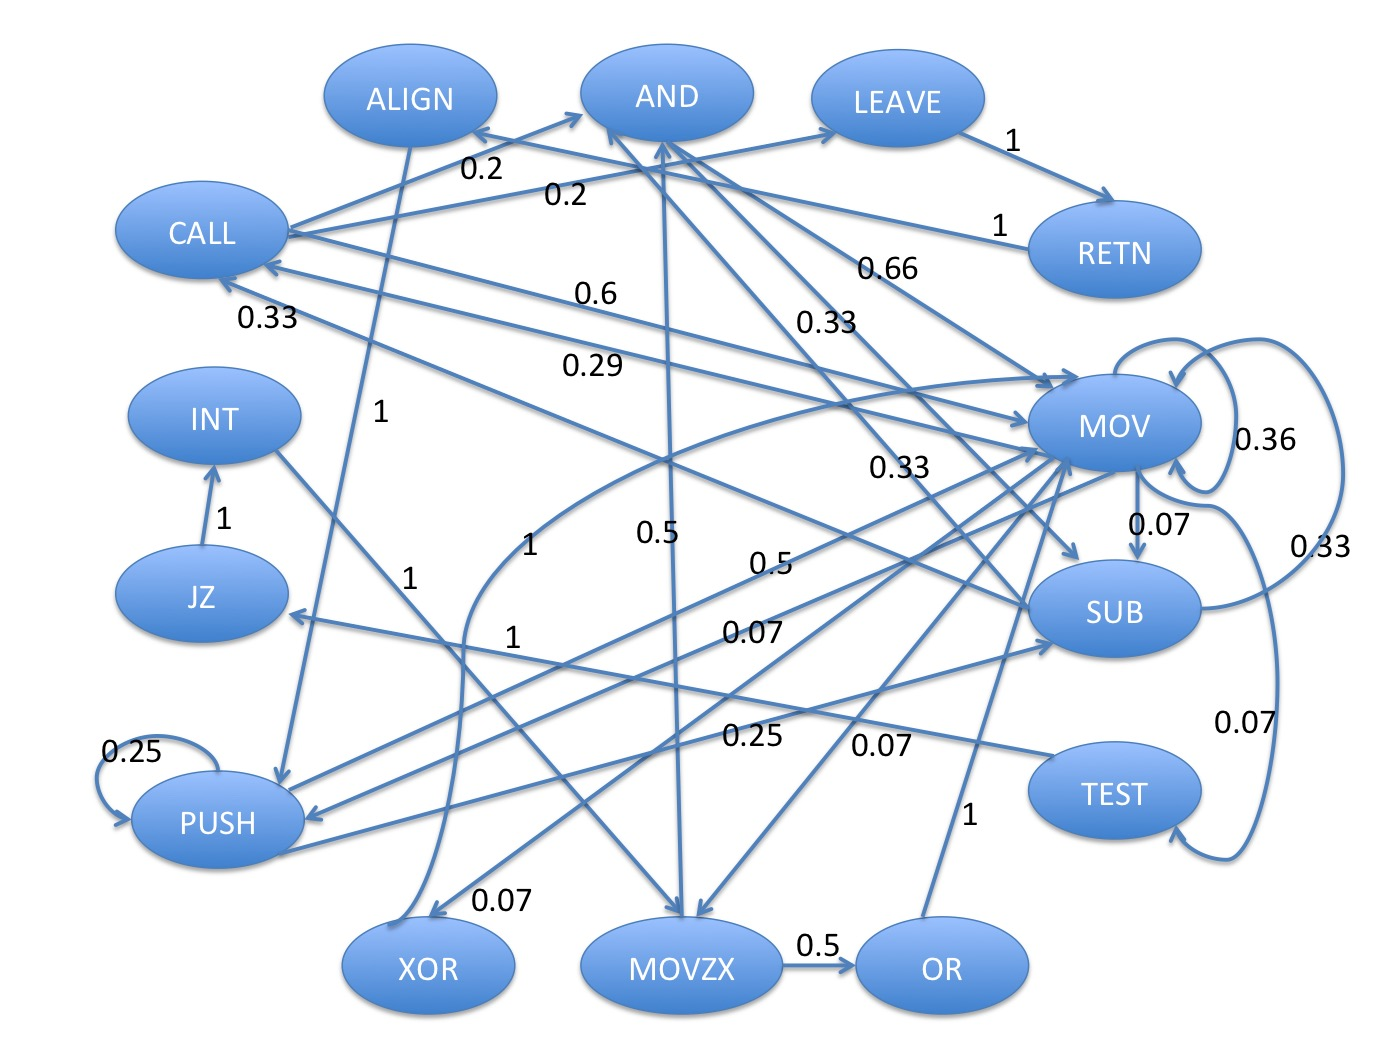
\includegraphics[width=16cm, height=12cm]{opcodegraph.jpg}
    \caption[Opcode Graph]{opcode graph for the probability matrix in Figure \cite{bib8}.}
    \label{fig:opcodegraph}
\end{figure}

\subsection{Similarity Score Calculation}  \label{opcodescorecalculation}
After creating probability matrices for the malware file and the test file, similarity between two files is calculated by taking the Manhattan distance between two probability matrices. Consider $A$ as the probability matrix of file 1 and each element in $A$ is denoted as $A_i,_j$ where $i$ and $j$ specifies $i^{th}$ row and $j^{th}$ column respectively. Similarly $B$ is the probability matrix of file 2 and each element in $B$ is denoted as $B_i,_j$. Similarity between matrix $A$ and $B$, is calculated as below \cite{bib8},

Similarity score = ${1 \over N^2}(\sum_{i,j=0}^{N-1}|a_i,_j-b_i,_j|^2)$ 

where N is total number of distinct opcodes present in the combination of both files.

Before using the similarity score, we have to determine the threshold score which distinguishes between benign files and malware files. The threshold value is determined as follows \cite{bib8},
\begin{enumerate}
\item Construct opcode graphs for all the variants of metamorphic malwares.
\item Construct opcode graphs for all the benign files.
\item Calculate the similarity scores for all pairs of malwares.
\item Calculate the similarity scores for every benign file against malware from step 1.
\item Determine a threshold value using the scores calculated in steps 3 and 4.
\end{enumerate}

\section{Transcriptase detection add-on structure}

\begin{figure}[h]
  \centering
\begin{lstlisting}[style=BashInputStyle,numbers=none,mathescape=false,tabsize=4,keywords=none]
Sravans-MacBook-Pro:TranscriptaseDetectionAddon sravan2j$ tree
.
|-- data
|  	  	  	  	   	|-- content-script.js
|  	  	  	  	   	|-- icon-16.png
|  	  	  	   	   	|-- icon-32.png
|  	  	  	  	   	|-- icon-64.png
|  	  	  	  	   	|-- java
|  	  	  	  	   	|  	  	  	  	   	|-- CheckOpcodes.class
|  	  	  	  	   	|  	  	  	  	   	|-- DownloadThread.class
|  	  	  	  	   	|  	  	  	  	   	|-- DownloaderApp.class
|  	  	  	  	   	|  	  	  	  	   	|-- GetScore.class
|  	  	  	  	   	|  	  	  	  	   	|-- ImageDownloader.class
|  	  	  	  	   	|  	  	  	  	   	|-- Lock.class
|  	  	  	  	   	|-- javaext.js
|  	  	  	  	   	|-- jquery-1.10.0.min.js
|  	  	  	  	   	|-- js.jar
|  	  	  	  	   	|-- malware_opcodes.txt
|  	  	  	  	   	|-- opcodes.bat
|  	  	  	  	   	|-- opcodes.sh
|-- lib
|  	  	  	  	   	|-- main.js
|-- package.json
|-- test
  	 |-- test-main.js
	
4 directories, 17 files
\end{lstlisting}
    \caption[Transcriptase detection add-on directory structure]{Transcriptase detection add-on directory structure}
    \label{fig:transdetectaddon}
\end{figure}
Figure~\ref{fig:transdetectaddon} shows the directory structure of Transcriptase detection add-on. 
\begin{enumerate}
\item "content-script.js" uses jQuery code to find the JavaScipt content in web page, so included "jquery-1.10.0.min.js" file in the "/data" directory to enable this functionality. 
\item "js.jar" helps the add-on to use the Rhino JS engine.
\item The Java files in the add-on are used to download the files, and to calculate the similarity score. All these files are placed in the "/data/java" directory.
\item "opcode.sh" is a shell script to invoke Java files. As shell scripts won`t work on Windows, the "opcode.bat" file is included to invoke Java files on Windows. 
\item The "malware\_opcodes.txt" file contains the opcodes of Transcriptase family malware. This file is used while validating web page JS content using the opcode graph similarity technique. 
\end{enumerate}
More details about these files are covered in subsequent sections.

\section{JavaScript extraction from web page}

As soon as the user enters a web page link, the browser loads the JavaScript content along with HTML and CSS on the page. Before extracting the JS from web page, we have to disable JS load in the browser to prevent the execution of JS malware code.

Enabling/disabling JS feature deals with browser preferences. The preferences system of Mozilla browser can be accessed using XPCOM interfaces like $nsIPrefService$ and $nsIPrefBranch$. The below code is used to disable JavaScript code,

\begin{figure}[h]
  \centering

\begin{lstlisting}[language=JavaScript] 
var prefSrv = this.prefService = Cc["@mozilla.org/preferences-service;1"]
                .getService(Ci.nsIPrefService);
var PBI = Ci.nsIPrefBranch2;
this.mozJSPref = prefSrv.getBranch("javascript.").QueryInterface(PBI);
this.mozJSPref.setBoolPref("enabled", false);
\end{lstlisting}
    \caption[Add-on code to disable JavaScript load on web page]{Add-on code to disable JavaScript load on web page.}
    \label{fig:disablejs}
\end{figure}

The code in Figure~\ref{fig:disablejs} is interpreted as follows: Line 1 in the above code retrieves the preference services of Mozilla. nsIPrefBranch2 interface, in line 2, allows the add-on to listen to the changes to preferences. Line 3 retrieves the "javascript" preference and queues nsIPrefBranch2 interface using QueryInterface(). Later, setBoolPref() method is used to disable the JS by setting "false" to "enabled". Similarly the below line of code enables JS load,
\begin{lstlisting}[language=JavaScript] 
this.mozJSPref.setBoolPref("enabled", true); 
\end{lstlisting}

After disabling JavaScript, as explained in Section ~\ref{sec:contentscript}, the content script i.e., "content-script.js", is used to extract JS. "content-script.js" uses jQuery element selector to find all the <script> elements and extract the JavaScript instructions contained in <script> tags as shown below:
\begin{lstlisting}[language=JavaScript,numbers=none,mathescape=false]
var code="";
$("script").each(function(){ 
    code=code+$(this).html();
});
\end{lstlisting}
Sometimes, JavaScript code is also placed in an external file and the location of the external JavaScript file is specified in the web page using a src attribute of a <script> element as shown below:
\begin{lstlisting}[language=JavaScript,numbers=none,mathescape=false]
<script src="external_javascript.js"></script>
\end{lstlisting}
There is a chance that this external files may contain JavaScript malware code, so using the code in Figure ~\ref{fig:extracturls}, all the external file`s URLs are extracted from the web page.
\begin{figure}[h]
  \centering
\begin{lstlisting}[frame=single,language=JavaScript,mathescape=false]
var baseUrl = window.location.protocol + "//" + window.location.host + "/";
var Urls = "";
var regex = new RegExp("^(?:[a-z]+:)?//", "i");
$("script[src]").each(function(){
  var sourceurl = $(this).attr("src");
  if(!regex.test(sourceurl))
  {
    Urls=Urls+baseUrl;
  }
  Urls=Urls+(sourceurl.replace(/^\/+/, ""))+"\n";
});
\end{lstlisting}
\caption[JavaScript to extract all the external script file URLs]{JavaScript to extract all the external script file URLs}
    \label{fig:extracturls}
\end{figure}
Following is the explanation of the code snippet in Figure ~\ref{fig:extracturls}:
\begin{enumerate}
\item "window.location.protocol" returns the protocol of the current web page URL along with colon(:). For instance, "http:", "https:", "ftp:". "window.location.host" returns the host name of the web page. For instance, the hostname of "http://www.somewebsite.com/tryit.jsp?filename=sample\_code" is "www.somewebsite.com". So, line 1 creates a base URL of the web page.
\item line 4 uses a jQuery element selector to retrieve the external file locations defined in src attribute of <script> tag.
\item line 6 uses regex to test whether the external files location is relative or absolute path.
\item Line 8 contains the logic for prepending the base URL to an external file location, if the external file location is relative path.
\item Finally, the "Urls" variable contains all the external local URLs, and these URLs will be saved in a temporary file.  
\end{enumerate}


Later, the add-on invokes the $opcodes.sh$ file as shown in Figure ~\ref{fig:invokeopcode}, which performs the following two functions:
\begin{description}
\item[Creates a temporary file] \hfill \\
"TmpD" returns the temporary directory location of the OS. In line 1, "opcodes.tmp" filename is concatenated to temporary directory path and getFile() method returns a nsIFile object referring to "<TMP\_DIR>/opcodes.tmp" location. Then createUnique() method creates the requested temporary file.
\item[Invokes opcode.sh] \hfill \\
The nsIProcess interface is used to execute a process. nsIProcess requires executable name to execute and if the executable file requires any parameters then these parameters need to be passed as args[] to the nsIProcess. 
\begin{enumerate}
\item Line 3 and 4 creates a nsIFile object referring to executable "/bin/sh". 
\item Line 5 and 6 creates an instance of process and initializes it to "/bin/sh" executable.
\item Line 7 and 8 adds both "opcode.sh" file path and temporary file path to "args" array. Then the process is executed using run() which executes the below command internally,
\begin{figure}[h]
  \centering
\begin{lstlisting}[frame=single,language=JavaScript,mathescape=false,numbers=none]
$ /bin/sh /Users/sravan2j/Downloads/TranscriptaseDetectionAddon/data/opcode.sh /tmp/opcodes.tmp
\end{lstlisting}
\caption[command that invokes opcode.sh internally]{command that invokes opcode.sh internally}
    \label{fig:invokeopcodeint}
\end{figure}
\end{enumerate}

\end{description}

\begin{figure}[h]
  \centering
\begin{lstlisting}[frame=single,language=JavaScript,mathescape=false]
Cu.import("resource://gre/modules/FileUtils.jsm");

// create a new tmp file
var file = FileUtils.getFile("TmpD", ["opcodes.tmp"]);
file.createUnique(Ci.nsIFile.NORMAL_FILE_TYPE, 0600);

var file = Cc["@mozilla.org/file/local;1"].
           createInstance(Ci.nsILocalFile);
file.initWithPath("/bin/sh");

var process = Cc["@mozilla.org/process/util;1"]
              .createInstance(Ci.nsIProcess);
process.init(file);

var args = ["/Users/sravan2j/Downloads/TranscriptaseDetectionAddon/data/opcode.sh"];
// append the tmp file to the parameters
args.push(tmpFile.path);
process.run(true, args, args.length);
\end{lstlisting}
\caption[add-on code to invoke opcode.sh]{add-on code that creates temporary file and invokes opcode.sh with temporary file}
    \label{fig:invokeopcode}
\end{figure}

\section{Purpose of the Shell script}

The opcodes.sh code, shown in Figure ~\ref{fig:shellscriptcode}, performs the following three functions:
\begin{enumerate}
\item Line 1 executes following Java files - $DownloadThread.class$, $DownloaderApp.class$, $ImageDownloader.class$, and $Lock.class$, to download all the external scripts. This java files uses multi threading approach to download all the external scripts in parallel which reduces the total download time.  
\item After the above step, the entire JavaScript content will be saved in the /tmp/JSStatements.js file. Line 2 takes the JSStatements.js file as input and generates opcodes for the JavaScript code in JSStatements.js using the Rhino JS engine. The output of this step is the "/tmp/opcodes.txt" file.
\item Line 3 executes CheckOpcodes java code which calculates the similarity score using the opcode similarity technique, between malware\_opcodes.txt and the opcodes.txt file. The output of this step is redirected to "\$1", which refers to the arguments passed to opcodes.sh. The bash command in Figure ~\ref{fig:invokeopcodeint} shows that the /tmp/opcodes.tmp file is passed as an argument while calling opcode.sh. 
\end{enumerate}

\begin{figure}[h]
  \centering
\begin{lstlisting}[frame=single,language=JavaScript,mathescape=false]
java -Xmx500m -cp "." data/DownloaderApp data/externalUrls.txt
java -cp "./data/js.jar" org.mozilla.javascript.tools.jsc.Main /tmp/JSStatements.js > /tmp/opcodes.txt
java -cp "./data" CheckOpcodes data/malware\_opcodes.txt /tmp/opcodes.txt > $1
\end{lstlisting}
\caption[opcode.sh shell script code]{opcode.sh shell script code}
    \label{fig:shellscriptcode}
\end{figure}

\section{Page validation and clean-up step}

The add-on gets the similarity score from the opcodes.tmp file. If the score is less than the threshold value i.e., 0.01, then the web page is considered as a malicious page or else it is a benign page. 
\begin{enumerate}
\item If the page is benign, then it enables JavaScript and reloads the web page.
\item If the page is malicious, then the web page won't be loaded; instead a prompt is displayed to the user regarding the malware.
\end{enumerate}
At the end, all the temporary files created will be removed as part of the clean-up step.

\section{Performance improvements} 
As the add-on performs lot of steps to validate the web page, the execution time will be more. So, instead of validating every web page every time, we can skip the validation during the following scenarios: 
\subsection{Fingerprinting web pages} \label{fingerprintingwp}
The hashcode of the benign web page should be saved in the user directory. In the future, when user visits the same web page and if the internal content of the page is not changed from the last visit, then the hash code of the page remains the same as the one that was saved on user`s machine. In this case, we can safely skip the validation of the web page. 

The disadvantage with this approach is that it consumes the user`s system memory as it saves the hashcode for every web page the user visits. 

We can also improve this approach by saving the hash codes in the cloud repository. Whenever any user visits the web page, the add-on connects with the cloud repository and checks if this web page was already validated by any user earlier or not. If it was validated, is the web page hash code the same? And what is the validation result? If the hash code is not in the cloud, then it will be validated by the current user`s plugin and the result will be stored in the cloud, so that this data will be useful for other users. Because of this approach, the user`s system memory will be saved and also at any point of time, the web page is validated only once by any user. Necessary security measures should be taken inorder to prevent the attacks like man-in-the-middle attack, cloud data tampering. 
 
\subsection{Whitelisting websites} 
Some popular websites are highly secured and regularly monitored, like Google, Facebook, Amazon etc. These websites can be added to benign page list by the user, so that they won`t be validated by the add-on.

The disadvantage of this approach is that it involves a risk of infection if the whitelisted web pages are infected by malware.

\section{Using other detection techniques} \label{otherdetecttech}
Currently this add-on uses only opcode graph similarity detection. Other detection techniques can be used in the add-on by simply changing line 3 of opcode.sh, shown in ~\ref{fig:shellscriptcode}, to execute a program that implements another detection technique instead of executing the CheckOpcodes program. The new program should accept "malware\_opcodes.txt" and "/tmp/opcodes.txt" as input files and the similarity score should be saved in the "/tmp/opcodes.tmp" file. No other changes are required. 